\documentclass[11pt]{article}

% ------- Enable UTF8 characters ------- %
\usepackage[utf8]{inputenc}
\usepackage[english]{babel}

\usepackage[toc,page]{appendix}

\usepackage{listings}
\usepackage{color}
\usepackage[colorinlistoftodos]{todonotes}
%\usepackage{pdfpages}

\usepackage{epstopdf}
\usepackage{wrapfig}
\usepackage{pdfpages}
\usepackage{todonotes}
\usepackage{multicol}
\usepackage{amsmath}
\usepackage{amssymb}
% ------------ Code Listing ------------- %

\definecolor{dkgreen}{rgb}{0,0.6,0}
\definecolor{gray}{rgb}{0.5,0.5,0.5}
\definecolor{mauve}{rgb}{0.58,0,0.82}

\lstset{frame=false,
  language=VHDL,
  aboveskip=3mm,
  belowskip=3mm,
  showstringspaces=false,
  columns=flexible,
  basicstyle={\small\ttfamily},
  numbers=left,
  numberstyle=\tiny\color{gray},
  keywordstyle=\color{blue},
  commentstyle=\color{dkgreen},
  stringstyle=\color{mauve},
  breaklines=true,
  breakatwhitespace=true,
  tabsize=3,
  moredelim=**[is][\color{mauve}]{@}{@},
}

% ------- Page layout ------- %
\usepackage{fullpage}
\usepackage{hyperref} % clickable references
\hypersetup{
    colorlinks,
    citecolor=black,
    filecolor=black,
    linkcolor=black,
    urlcolor=black
}
\usepackage{multicol}
\setlength{\columnsep}{1cm}

% ------- Images ------- %
\usepackage{graphicx}
\usepackage{caption}
\usepackage{float}
\usepackage{subcaption}
\DeclareCaptionFont{gray}{\color{gray}}
\captionsetup{textfont={footnotesize,sc,gray},font={footnotesize,sc,gray}}

\usepackage{blindtext}

% Test

\usepackage{tikz}
\usetikzlibrary{shapes,arrows,shadows}
\newcommand{\mx}[1]{\mathbf{\bm{#1}}} % Matrix command
\newcommand{\vc}[1]{\mathbf{\bm{#1}}} % Vector command

\begin{document}
\begin{titlepage}
\newcommand{\HRule}{\rule{\linewidth}{0.5mm}} % Defines a new command for the horizontal lines, change thickness here

\center % Center everything on the page
 
%----------------------------------------------------------------------------------------
%	HEADING SECTIONS
%----------------------------------------------------------------------------------------

\textsc{\LARGE University of Southern Denmark}\\[1cm] % Name of your university/college
\textsc{\Large SML (F16)}\\[0.3cm] % Major heading such as course name
\textsc{\large Statistical machine learning }\\[0.3cm] % Minor heading such as course title
\vspace{0.5cm}
\begin{figure}[H]
\centering

\includegraphics[scale=1]{img/sdu-segl.png}
\end{figure}
\vspace{0.4cm}
%----------------------------------------------------------------------------------------
%	TITLE SECTION
%----------------------------------------------------------------------------------------

\HRule \\[0.4cm]
{ \huge \bfseries SML - Final Report}\\[0.4cm] % Title of your document
\HRule \\[1.5cm]
 
%----------------------------------------------------------------------------------------
%	AUTHOR SECTION
%----------------------------------------------------------------------------------------

\begin{minipage}{0.4\textwidth}
\begin{flushleft} \large
\emph{Author:}\\
Mikael \textsc{Westermann}\\
\url{miwes12@student.sdu.dk}\\
Keerthikan \textsc{Ratnarajah}\\ % Your name 
\url{kerat12@student.sdu.dk}
\end{flushleft}
\end{minipage}
~
\begin{minipage}{0.4\textwidth}
\begin{flushright} \large
\emph{Lecturer:} \\
Prof. Norbert \textsc{Krüger}\\ % Supervisor's Name
\url{norbert@mmmi.sdu.dk}\\
\emph{Supervisor:} \\
Ph.d. Stud. Troels Bo \textsc{Jørgensen}\\
\url{trjoe@mmmi.sdu.dk}
\end{flushright}
\end{minipage}\\[4cm]

% If you don't want a supervisor, uncomment the two lines below and remove the section above
%\Large \emph{Author:}\\
%John \textsc{Smith}\\[3cm] % Your name

%----------------------------------------------------------------------------------------
%	DATE SECTION
%----------------------------------------------------------------------------------------

{\large \today}\\[3cm] % Date, change the \today to a set date if you want to be precise

%----------------------------------------------------------------------------------------
%	LOGO SECTION
%----------------------------------------------------------------------------------------

%\includegraphics{Logo}\\[1cm] % Include a department/university logo - this will require the graphicx package
 
%----------------------------------------------------------------------------------------

\vfill % Fill the rest of the page with whitespace

\end{titlepage}
\tableofcontents
\newpage
\listoffigures
\newpage
\section{Introduction}
<<<<<<< HEAD
\todo[inline]{Something...}
The purpose of this report is to develop a system capable of recognizing hand writting characters such as digits (0 - 9).  This report will contain different approaches of classifying this, and their performance.  The dataset used for training and testing the performance of this, has be been made by the students of the statical machine learning class  as seen in \ref{fig:data}. The dataset consist of 400 $\times$ 10 individually handwritten numbers,  provided by each  student of the class.  

\begin{figure}[H]
\centering
\includegraphics[width =0.6\textwidth]{../../SML-database/2016/group2/member1/Ciphers100-0.png}
\caption{Example of the  dataset}
\label{fig:data}
\end{figure} 

The process of recognizing the digits can be divided into 3 steps. 
\begin{itemize}
\item Preprocessing - Extracting the data, and discard irrelevant information. 
\item Feature extraction - Extracting relevant features 
\item Classification - Use the extracted to classify the digits. 
\end{itemize}

=======
>>>>>>> 34ff1c3365fe38aae75203e9098a9fe6bb020ed5

\chapter{kNN}
K - nearest - neighbor or kNN,
is a method for classifying objects based on the distance
to features extracted from ones training data.
The idea in kNN is to identiy k observation which is closest to the new
observation trying to be classified.
 The class with most vote determines which class the new observation
will be classified as. 
K is arbitrarily choosen by the user,
 and has an effect of the peformance of the algorithm. 
k-nn has an optimal classification rate when k becomes very large, 
but will computation wise take more time and vice versa. 
\section{SVM}
Support vector machines is a supervised learning method that analyzes the data and tries to recognize patterns, within the classification domain. The standard SVM method is an binary classifier, which predicts for a given input which class the input belongs two. Prediction is done based on the model it builds from the training session, the model provides a "clear gap" that provide the distinction between the first or the latter class. \\

Support vector machine constructs a hyperplane or set of hyperplanes in a high dimension. The hyperplane that has the largest distance to the nearest training data points of any class (so-called functional margin), provides the best separation,  since it result it a clear distinction between the classes, and lower general error.
\\

The goal in SVM is to find this hyperplane which provides the optimal separation of the classes by having the widest margin. 

\begin{figure}[H]
\centering
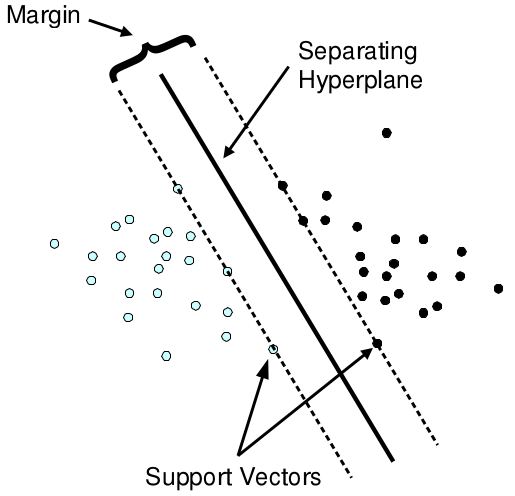
\includegraphics[width = 0.5\textwidth]{img/SVM-illu.png}
\caption{Svm Illustrated}
\label{fig::SVM-illustrated}
\end{figure}

The training data for this method consist a set of input vectors denoted as $\mathbf{x_i}$, each input vector has a number of component features. Each input vector is given a label, indicating its class.

The hyperplane is given as 
\begin{equation}
\mathbf{w} \cdot \mathbf{x} + b = 0
\end{equation}

In which the $\mathbf{w}$ determines the orientation of the plane, and $\mathbf{b}$ is the offset of the plane from the origin. \\
 
The seperaing hyperplane which maximizes the margin can be found by examining the convex hull of each class’s training data  and then find the closest points in the two convex hulls. The convex hull of a set of points is the
smallest convex set containing the points.  If the hyperplane that bisects both convex hulls can be found, will the resulting classifier deemed robust in some sense. 

\begin{figure}[H]
\centering
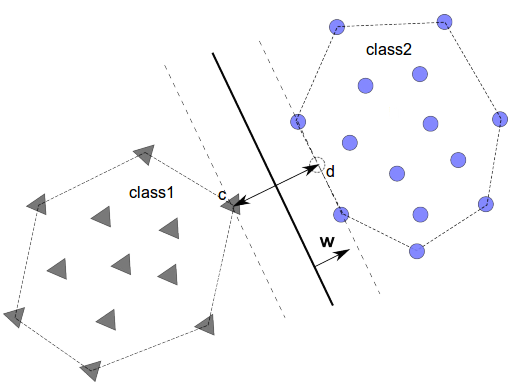
\includegraphics[width = 0.5\textwidth]{img/convex_hull.png}
\caption{best plane bisects closest points in the convex hulls,The convex hulls are labeled c and d}
\label{fig::convex_hull}
\end{figure}  

To find  the plane, one have to find the points closest to the plane, which can be found by solving the quadratic problem. \\ 

\begin{equation}
min_\alpha~\left(\frac{1}{2} ||c-d||^2\right)
\end{equation}

where c and d are the closest to be found points, these are defined as 
\begin{equation}
\begin{aligned}
&c = \sum_{y_i~\in~class1} \alpha_ix_i  
& \text{subject to}
&& \sum_{y_i~\in~class1}\alpha_i =1 
&& \alpha_i \geq 0
\end{aligned} 
\end{equation}

\begin{equation}
\begin{aligned}
&d = \sum_{y_i~\in~class2} \alpha_ix_i  
& \text{subject to}
&& \sum_{y_i~\in~class2}\alpha_i =1 
&& \alpha_i \geq 0
\end{aligned} 
\end{equation}


An alternative approach involves a search through the space of every possible hyperplane in order to find a set of two parallel planes that divide the points into homogeneous groups yet themselves are as far apart as possible.\\


In the case of non-linearly separable data, can a linear hyperplane not be used to define the solution. For this purpose is a slack variable introduced, which allows some points on the incorrect side of the margin, creating a soft margin, when a linear hyperplane was used to separate them.\\

A different approach for solving this problem would be using the kernel trick. The kernel trick involves transforming in $\mathbb{R}^n \rightarrow \mathbb{R}^{n+1}$. The challenging part is to find such transformation, $\phi$ which allow transforming data into a higher dimension. 

Kernel functions are in general in the following form:
\begin{equation}
K(\overrightarrow{x_i},\overrightarrow{x_j}) = \phi(\overrightarrow{x_i}) \cdot \phi(\overrightarrow{x_j}) 
\end{equation}

$x_i$ and $x_j$ illustrates two different feature vectors. 

Different kernels does already exist, and may already be implemented in different SVM software packages. 

\textbf{Linear kernel}:
\begin{equation}
K(\overrightarrow{x_i},\overrightarrow{x_j}) = (\overrightarrow{x_i}) \cdot (\overrightarrow{x_j}) 
\end{equation}

Linear kernel does not transform the data, but computes the dot product. 

\textbf{Polynomial kernel of degree $d$}:
\begin{equation}
K(\overrightarrow{x_i},\overrightarrow{x_j}) = ((\overrightarrow{x_i}) \cdot (\overrightarrow{x_j})+1)^d
\end{equation}

The Polynomial kernel adds a nonlinear transformation of the data.


\textbf{Sigmoid kernel}
\begin{equation}
K(\overrightarrow{x_i},\overrightarrow{x_j}) = tanh( k(\overrightarrow{x_i}) \cdot (\overrightarrow{x_j}) - \delta)
\end{equation}

The choice of kernel depends what kind of transformation is needed. 
\chapter{PCA - Principal Component Analysis}
PCA is a tool used to find a low dimensional representation of a data set that represent as much variation as the complete data set.   The analysis finds uncorrelated variables named principal components from the dataset.  Using PCA would therefore also help lessen the change of "curse of dimensionality", and also improve the time needed to process the data. 

\begin{figure}[H]
\centering
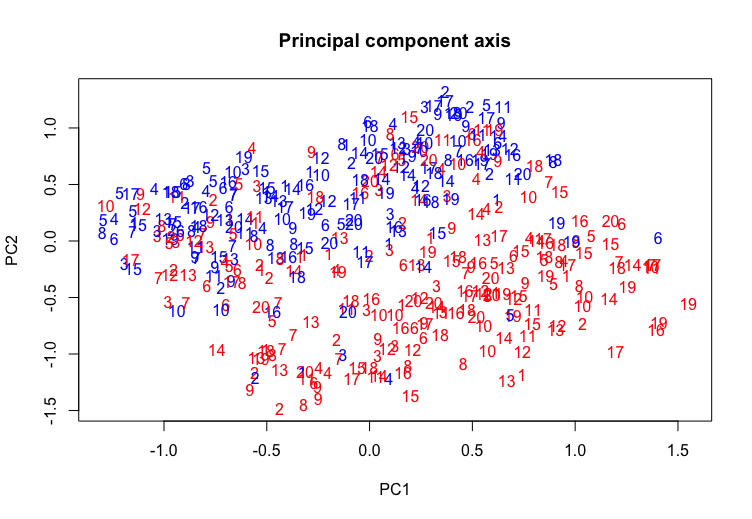
\includegraphics[width = \textwidth]{Figure/PCa-axis.png}
\caption{ red numbers indicated the axis of PC1 and the blue numbers determine the axis of PC2}
\label{fig:pca_vis}
\end{figure}

An illustration of the first two principal components of person dependent dataset can be seen in figure \ref{fig:pca_vis}. The axis shows how the data is distributed along both axis.  It shows that the PC1 axis has the greatest, as it can be seen from the variance of data aswell. 
\\
\\
As more PC gets included, will more of the variation of the dataset be exploited, and at the end completely resemble the the original data. The trick here is to find the right amount of PC which exploits the dataset as much as possible, and reduce the "unwanted" dimensions in the dataset. 

\begin{figure}[H]
\centering
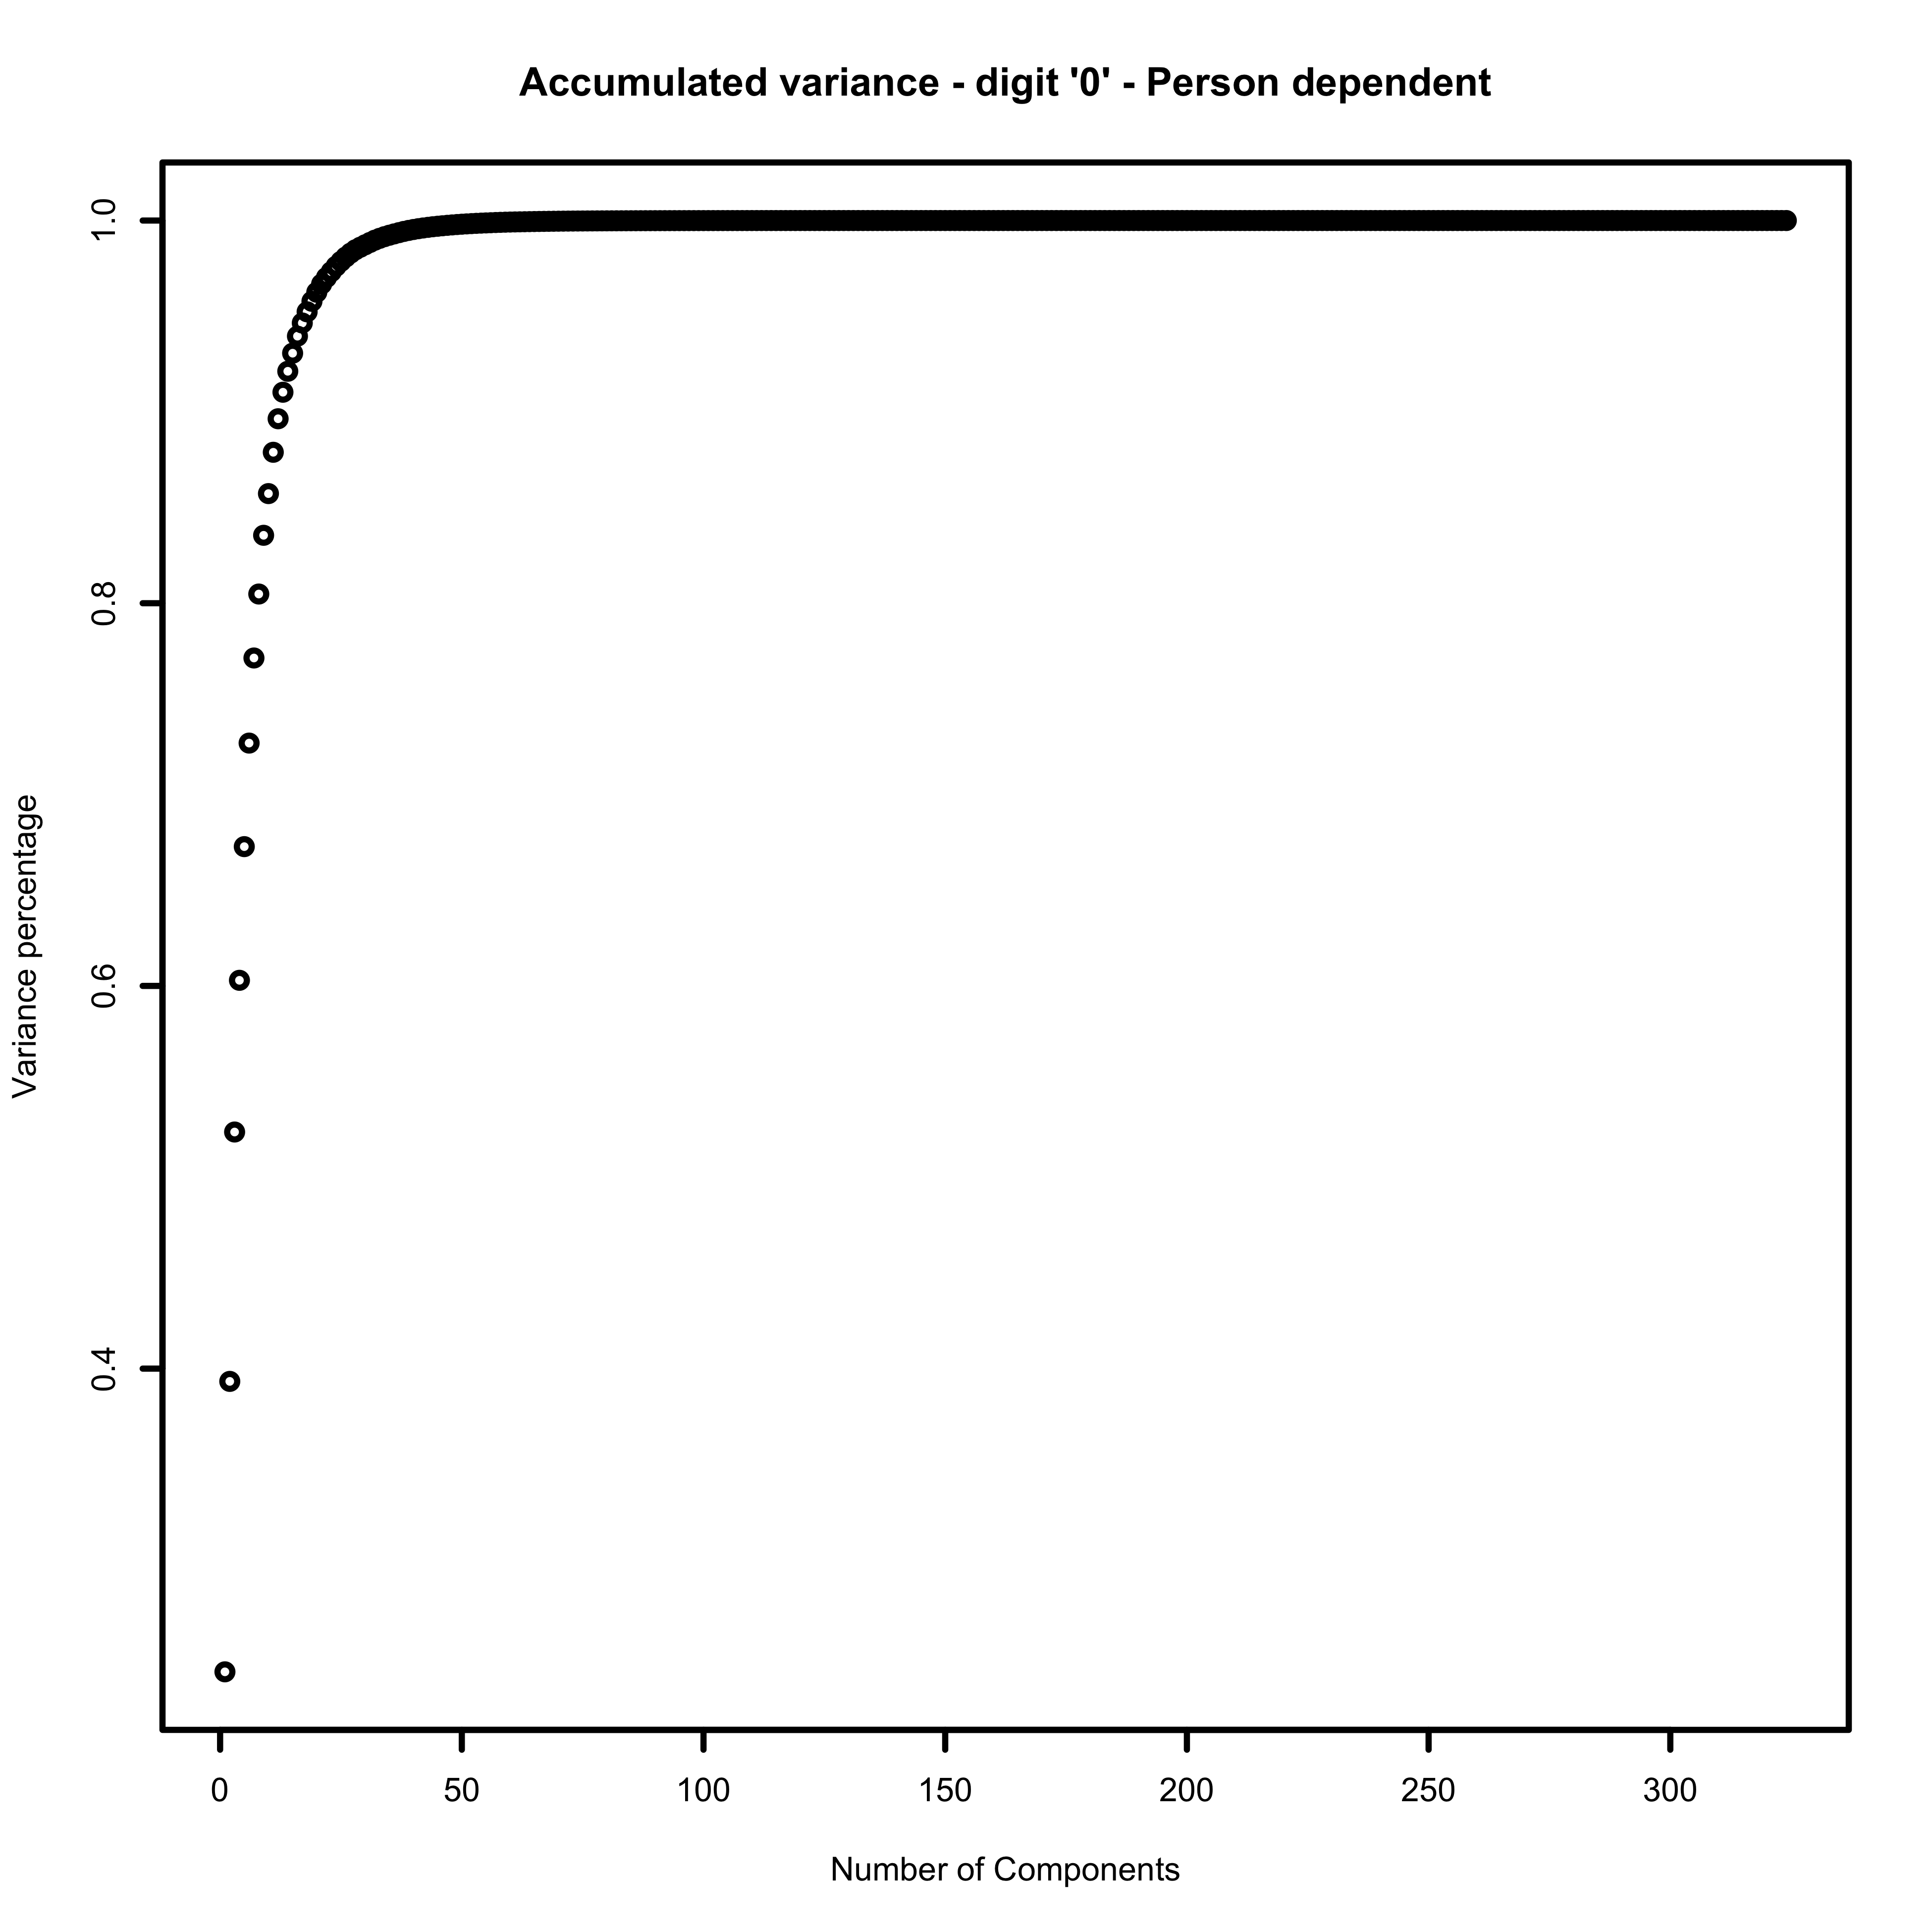
\includegraphics[width = 0.8\textwidth]{Figure/accumulated-2-1-person-dependent.png}
\caption{Plot showing the variance being accumulated for each component}
\label{fig:PCa_num_comp}
\end{figure}

As it can be seen in figure \ref{fig:PCa_num_comp} increased the accumalted variance strongly for the first principal components.  Using the elbow method one would be able to determine how many would be to determine how many would pc would fairly represent the dataset. 
\\
\\
\\
Using the PCA method were the dataset reduced into 4 sets  which represents 80\% , 90\%, 95\%, 99\% variances. The training was trained using a 10 - fold cross validation, which was repeated 10 times, and the accuracy mean was then computed. 

\begin{figure}[H]
\centering
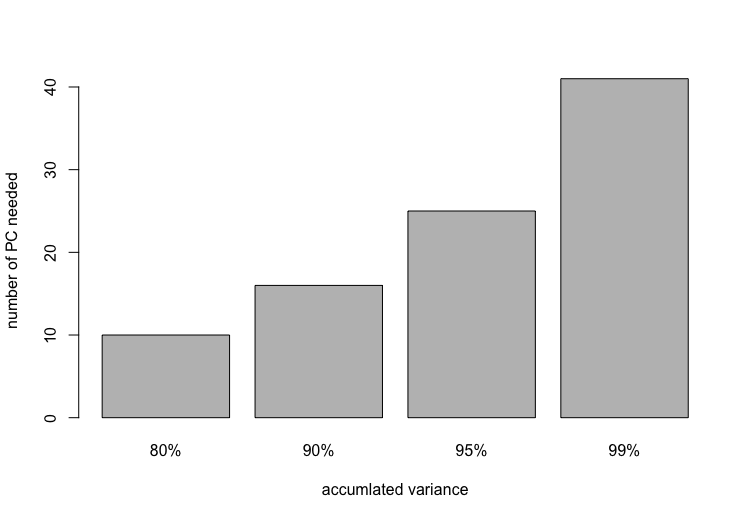
\includegraphics[width = \textwidth]{Figure/PCA_barplot.png}
\label{fig:pca_comp}
\caption{The number of components needed to achieve the desired variance}
\end{figure}

Using the PC were knn performed which resulted in this

\begin{figure}[H]
\centering
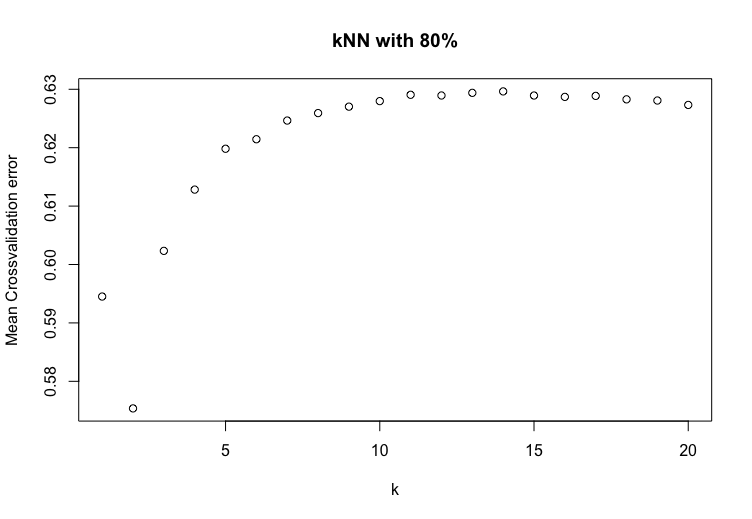
\includegraphics[width = \textwidth]{Figure/kNN_plot_80.png}
\label{fig:knnFit_80}
\end{figure}

\missingfigure{KnnFit Confusionmatrix}

\begin{figure}[H]
\centering
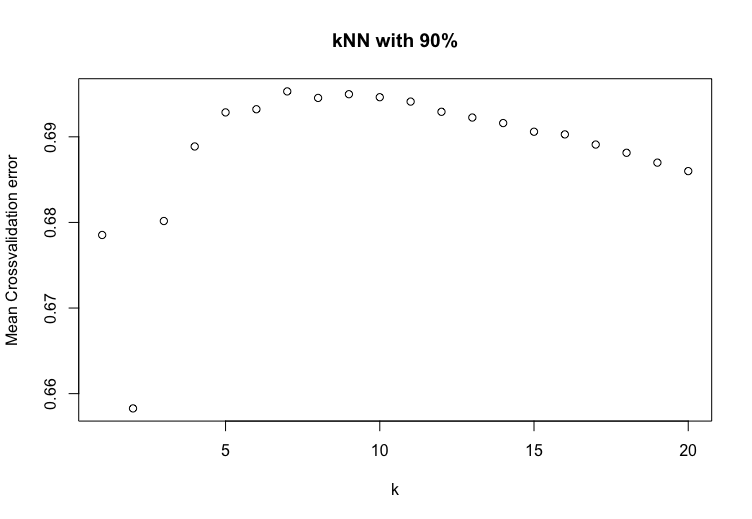
\includegraphics[width = \textwidth]{Figure/kNN_plot_90.png}
\label{fig:knnFit_90}
\end{figure}


\begin{figure}[H]
\centering
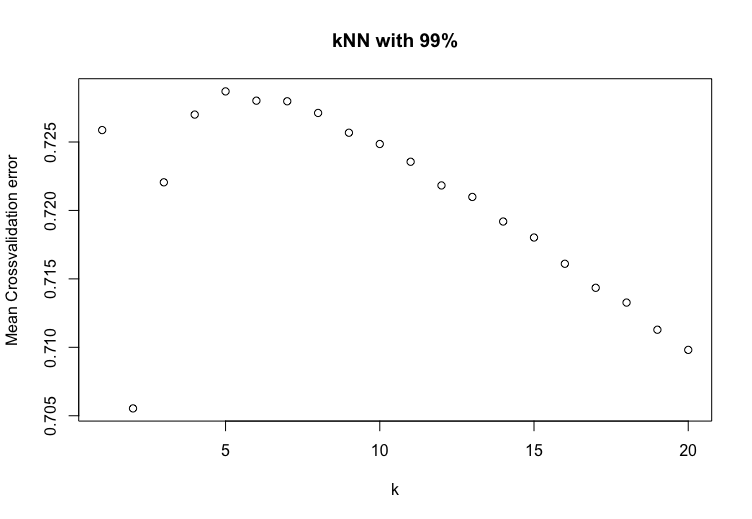
\includegraphics[width = \textwidth]{Figure/kNN_plot_99.png}
\label{fig:knnFit_99}
\end{figure}


\missingfigure{KnnFit plots}


\missingfigure{knnFit trainingTime}


\todo[inline]{prediction time.}
\section{Preprocessing}
This section will entails details about the preprocessing step, what have been done to the scanned images, and why it has been done. 
\section{Analysis}
This section will entail the training and testing phase of both methods. The two 
algorithm has to applied to three different digit recognition problems, they 
being 
\begin{itemize}
\item	Data from a single person
\item	Data from all persons with a training set that includes data from all 
persons.r
\item Data from all persons where the training set does not include data from 
the persons in the test set.
\end{itemize}

\subsection{Test with Data from single person}
\label{sec::test_with_data_from_single_person}

The first training were conducted with every single persons training set. The 
training using kNN consisted of k = 5,with a 10 - fold cross validation. k = 5 
was chosen, as it was previously shown (see other sections...\todo[inline]{make 
section 
stating this}) to provide the highest accuracy on the other dataset. \\

The training using SVM were performed using a polynomial kernel, with a degree 
of 2, scale of 0.1   and cost of 0.5 with a 10 fold cross validation as well. 
The polynomial kernel was chosen due to prior experiments with other kernel, and 
had a higher degree of freedom would provide a better accuracy.\\ 
\todo[inline]{maybe a bit fluffy idk?}

 
A
10-fold cross validation uses 1 fold for testing and the rest for training 
purposes it thereby provides an average of the accuracies on how well a trained 
classifier, trained using the persons own data is capable of detecting himself.  
This information provides some insight on how consistent the persons writing is. 
An inconsistent writing style will cause lower mean accuaracy compared to a 
consistent style. \\

 Each accuracy is given an error bar stating the standard deviation of the 
dataset. The standard deviation of the mean accuracy is found by adding the 
internal standard deviation and the external standard deviation. The internal 
standard deviation is a vector of all individual standard deviation acquired 
from the 10-fold cross validation, an the external consist of the variance 
between the accuracies acquired  from the 10-fold cross validation. 
 
 The result of this test can be seen here...
 
 \missingfigure{The great plot! single person test kNN/svm - Kiddi sucks at 
writing plot :(}

\subsection{Test with data from all persons with a training set that includes 
data from all}


 

\subsection{Test with Data from all persons where the training set does not 
include data from 
the persons in the test set}






\section{Discussion}
\section{Conclusions}
\label{sec:conclusion}
%The main purpose of this project is to compare two classification algorithms,
%k-Nearest Neighbours (k-NN) and Support Vector Machines (SVM),
%for handwritten digit recognition.
%The second purpose of this project is to achieve good classification performance,
%and thus, some preprocessing is needed.
%Lastly, as the digits used in this project
%were written by a class of 23 always competitive students,
%it was chosen to estimate the quality of the hand written digits
%and identify the student with the worst hand writing.
%This required a definition of hand written digit quality,
%which is also presented here.
k-NN with number of neighbours k=5 achieves significantly higher overall 
classification accuracy than SVM with polynomial kernel of degree 2
with scale factor 0.1 and cost of constraints violation C=0.5,
with \(\alpha=0.05\),
when each algorithm is trained with a dataset of hand written digits
from a class of 23 people, and tested on a dataset
with digits written by the same people.
When the training set only contains data from 22 people,
and the test set is written by a person not in the training
set, k-NN does not perform significantly worse
than SVM, although a lower overall accuracy was observed.
Neither does the k-NN classifier perform significantly worse than SVM
when applied to one persons data at a time,
although a lower overall accuracy was observed.

The highest obtained overall classification accuracy is 0.854 with a standard
deviation of 0.0205, for the SVM classifier.

A successful preprocessing scheme involving the perspective transform,
gaussian blur and Principal Component Analysis was implemented.

Person \(G2M1\) (one of the authors) has the worst digit hand writing of the 2016 SML class,
when the writing quality is measured by classification
error on own data. This means \(G2M1\) has the least
within-digit consistent and between-digit varied
hand writing.
\end{document}

